\section{Grachten}

Problem summary: given three lengths $AB$, $AC$, $BD$ forming the base and partial
lengths for the adjacent side and hypotenuse, determine the remaining length of the
adjacent side.

\begin{center}
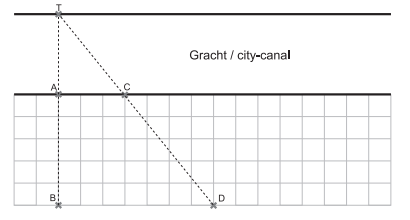
\includegraphics[scale=0.75]{f_diagram.png}
\end{center}

Let the goal length be known as $x$. If we consider the point $B$ to be the origin,
then we can use the provided lengths to determine the equation of the line for the
hypotenuse. The two points $C$ and $D$ can be represented as follows: \\

\begin{center}
$C = (AC, AB)$, $D = (BD, 0)$  
\end{center}

Finding the gradient of the line $CD$ gives us: 

$$
\begin{aligned}
m &= \frac{-AB}{BD - AC}
\end{aligned}
$$

Which we then use to find the equation of the line, solving for the y-intercept by
substituting in $D_x$ which will always give $y = 0$.

$$
\begin{aligned}
y &= mx + c \\
0 &= \frac{-AB}{BD - AC} \cdot BD + c \\
c &= \frac{AB}{BD - AC} \cdot BD \\
\end{aligned}
$$

Finding the length $x$ then becomes a simple matter of subtracting $AB$ from $c$:

$$
x = c - AB
$$

To convert this decimal answer into the appropriate format we used David Eppstein's
rational approximation for real numbers, using the theory of continued fractions. 
The runtime for this approximation is $O(d)$ where $d$ is the maximum denominator
allowed.

\vspace{0.5cm}
Overall this runs in $O(1)$ time and memory.
